\subsubsection{Single Execution Time Measurement}\label{sec:qe_time}

\begin{figure}[th]\centering
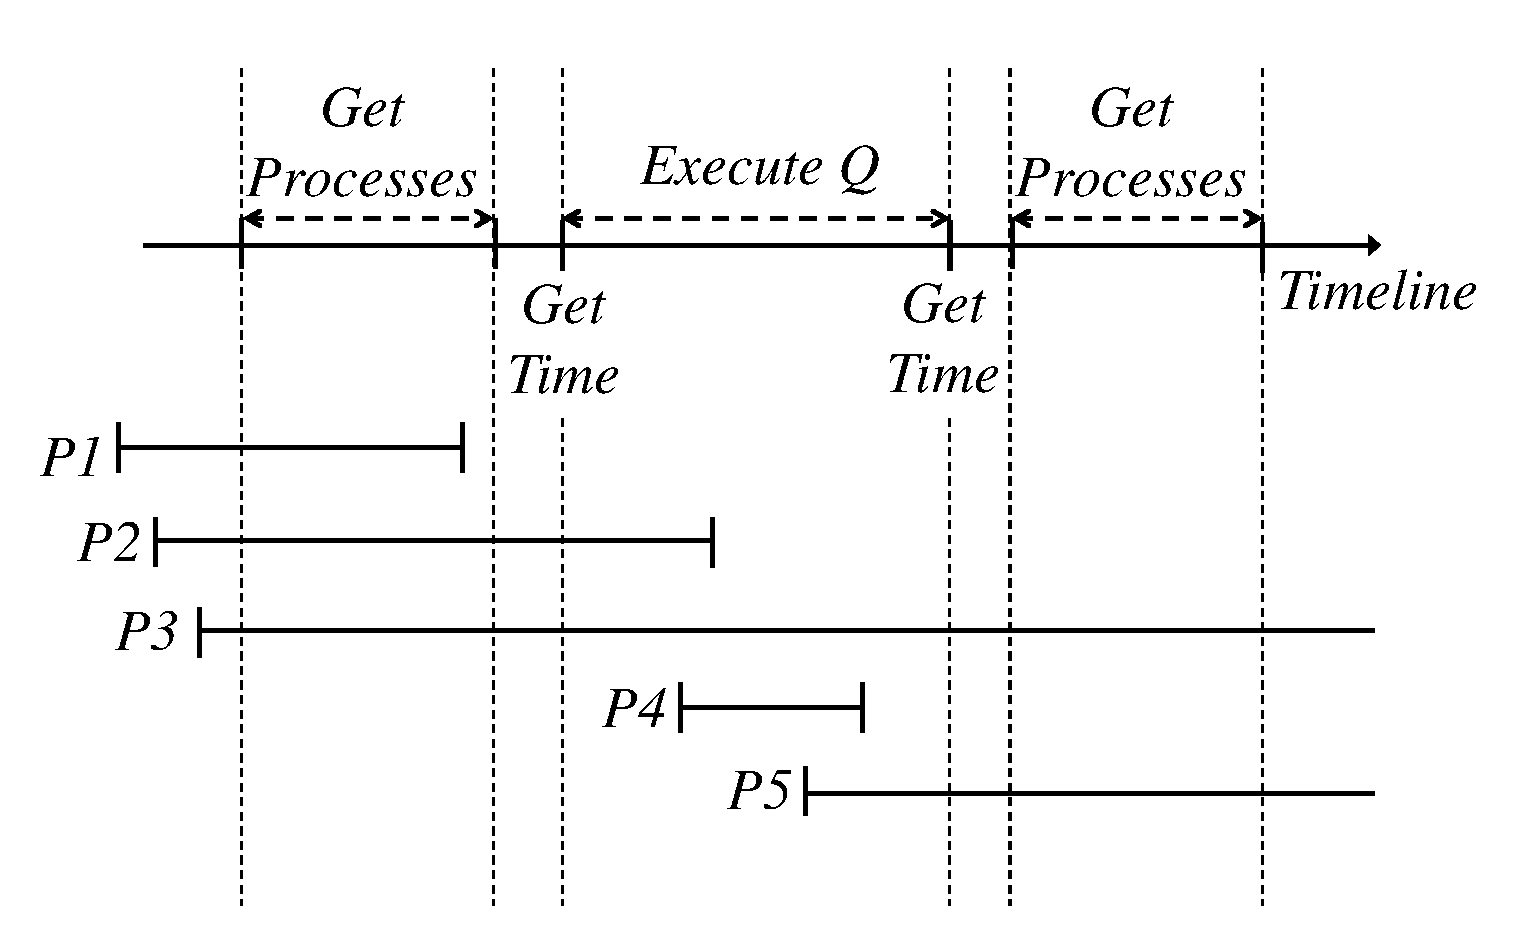
\includegraphics[width=0.50\textwidth]{figures/time_measurement.eps}
\caption{Processes influencing query execution\label{fig:timing}}
\end{figure}

In this section we discuss how we measure query execution time. 
As illustrated in Figure~\ref{fig:timing}, 
we first get all running processes before executing 
a query $Q$. 
Then timer for $Q$ gets started, and it is stopped after $Q$ gets 
executed. 
The execution time for $Q$ is measured by the time difference, and 
we finally finish single query execution by examining running 
processes right after the execution. 

Now let us examine how other processes may influence query execution. 
Assume that all the processes below are not relevant to DBMS processes.
Before timing $Q$, processes $P$1, $P$2 and $P$3 are recorded into 
a map $M$1. 
Another map $M$2, on the contrary, keeps processes $P$3 and $P$5 
captured after the timing. 
For each recorded process, the maps $M$1 and $M$2 keep 
$<$process id (pid), \{process name, minimum/major faults, 
cpu/system times\}$>$. 
The cpu and system times are considered for the subtraction. 
The process information can be achieved by iterating 
{\tt /proc/\{pid\}/stat} associated with each process. 

By comparing $M$1 and $M$2, we easily know that $P$3 and $P$5 affected 
$Q$'s execution; thus, the time spent on $P$3 and $P$5 are subtracted from 
the measured query execution time. 
$P$1 and $P$2 that do not appear in $M$2 must have stopped 
before or during the query execution, respectively. 
We cannot determine whether the query execution is affected by 
these stopped processes. 
For instance, $P$2 is explicitly involved with the execution whereas 
$P$1 not. 
What we can know is that regarding the execution, there were stopped 
processes, such as $P$1 and $P$2, as a result of comparison with 
$M$1 and $M$2. 
This execution, therefore, will be thrown out due to the stopped ones. 

Note that $P$4 is a {\em phantom} process, since it does appear 
in neither $M$1 nor $M$2. 
The existence of phantom process can be known by comparing 
the number of processes from {\tt /proc/stat} before and after execution.
Like stopped processes, we throw out any execution with a phantom process, 
considering measurement accuracy.

\begin{figure}[t]
\begin{center}
\begin{algorithmic}
{\bf Algorithm} timeSingleQueryExecution($i$, $q$, \\
						\hspace{44.0mm}$exPlan$, $card$):
\STATE $plan$ $\leftarrow$ get(Prepared)QueryPlan($q$)
\IF{$plan$ $\neq$ $exPlan$}
	\STATE Error: two different plans are observed \\ 
	at the same cardinality. \\
\ENDIF
\STATE Flush disk drive/OS/DBMS caches. \\
\STATE $M1$ $\leftarrow$ $extractAllRunningProcs$() \\
\STATE $startTime$ $\leftarrow$ $getCurrTimeMills$() \\
\STATE $executeQuery$($q$) \\ 
\STATE $endTime$ $\leftarrow$ $getCurrTimeMills$() \\	
\STATE $execTime$ $\leftarrow$ $endTime$ - $startTime$ \\	
\STATE $M2$ $\leftarrow$ $extractAllRunningProcs$() \\
\STATE $procDiff$ $\leftarrow$ $diff$($M1$, $M2$) \\	
\STATE RecordQueryExecution($i$, $q$, $card$, \\ 
			\hspace{34.0mm}$execTime$, $procDiff$) \\
\end{algorithmic}
\caption{Timing single query excution\label{alg:timing}}
\end{center}
\end{figure}
